\documentclass[12pt]{article}
\usepackage[a4paper,margin=1in]{geometry}
\usepackage{times}
\usepackage{setspace}
\usepackage{hyperref}
\usepackage{booktabs}
\usepackage{enumitem}
\usepackage{float}
\usepackage{url}
\usepackage{graphicx}
\setstretch{1.0}

\title{Reimplementation of the MapReduce Mechanism Using Go}
\author{
Anyi Jia \quad Peiyang Li \quad Jiarun Zheng\\
City University of Hong Kong\\
Group ID: \texttt{[Group 345]}
}


\begin{document}
\maketitle

\begin{abstract}
This project reimplements the core MapReduce execution model in Go and validates it with a word-count workload. Our system follows a master-worker architecture and uses Go RPC over TCP for coordination. The master manages map and reduce task states, assigns work dynamically, and reassigns timed-out or failed tasks. Workers load user-defined map/reduce logic from a Go plugin, execute tasks, persist intermediate key-value pairs as JSON files, and emit final outputs after the reduce phase.

Compared with a monolithic sequential implementation, this design exposes the key mechanisms of practical distributed data processing: task scheduling, synchronization, intermediate data partitioning, and basic fault tolerance. We deployed the implementation with one master and multiple workers and tested it on multiple text files from Project Gutenberg. Results show that the framework can complete the full map-shuffle-reduce pipeline correctly and recover from worker-side failures/timeouts by reallocation.

The project demonstrates how Go's concurrency-friendly ecosystem can be used to build an educational MapReduce runtime with clear modular boundaries. We also provide an artifact appendix including dependency requirements, build instructions, execution scripts, and expected outputs for reproducibility.
\end{abstract}

\section{Introduction}
MapReduce is a classic programming model for scalable data processing. It hides distribution complexity behind two user functions: \texttt{Map} transforms input records into intermediate key-value pairs, while \texttt{Reduce} aggregates values by key. Since its introduction, MapReduce has influenced many large-scale data systems.

The goal of this project is to reimplement key MapReduce mechanisms from scratch in Go rather than only using an existing framework. This makes the execution logic transparent: task lifecycle control, worker-master coordination, intermediate file organization, and recovery under partial failures. Following our proposal, we focus on a technical reimplementation with deployable software artifacts.

Our method is implementation-driven. We design a centralized master that tracks state for all map/reduce tasks, and decentralized workers that repeatedly request tasks, execute them, and report status. We use plugin-based \texttt{Map}/\texttt{Reduce} functions to keep the runtime generic. We evaluate the system with the WordCount application and discuss behavior under normal and failure-prone runs.

\section{MapReduce Principle and Design Rationale}
\subsection{Execution Model}
This project follows the classic two-stage model: map first, reduce second. Each input text file is treated as one map task, and the number of reduce tasks is fixed by \texttt{NReduce}. Workers do not receive pushed tasks from the master; instead, they continuously pull work by RPC (\texttt{AskForTask}). This pull model simplifies elastic worker participation because the master only needs to track task states, not long-lived worker identities.

\subsection{Task-Worker Relationship}
Following the lab principle, there is no permanent one-to-one binding between a worker and a specific task type. A worker can execute different map or reduce tasks at different times, or remain idle when no task is immediately available. This design improves robustness under churn: if a worker exits or stalls, the system can continue as long as another worker can pull pending work.

\IfFileExists{assets/images/MapReduce_relation.png}{
\begin{figure}[H]
\centering
\includegraphics[width=0.95\textwidth]{assets/images/MapReduce_relation.png}
\caption{Principle-level interaction: workers repeatedly pull tasks from the coordinator, execute map/reduce jobs, and return status; the coordinator centrally tracks task state and phase progression.}
\label{fig:principle-relation}
\end{figure}
}{}

\subsection{Intermediate Data Routing Principle}
The framework uses deterministic partitioning: a key is routed to a reduce bucket by \texttt{ihash(key) \% NReduce}. Therefore, identical keys from different map tasks always converge to the same reduce task. Intermediate files are named in the form \texttt{mr-out-mapId-reduceId}, and reduce task \texttt{r} scans files matching \texttt{mr-out-*-r}. This naming-and-hashing contract is the core guarantee for correct grouping semantics.

\subsection{Failure and Timeout Semantics}
The coordinator handles two failure classes:
\begin{itemize}[leftmargin=1.5em]
  \item \textbf{Explicit failure:} a worker reports \texttt{MapFailed}/\texttt{ReduceFailed}.
  \item \textbf{Implicit failure:} a running task exceeds a timeout threshold and is considered lost.
\end{itemize}
In both cases, the task becomes reassignable. This matches the lab's practical assumption: duplicate completion reports may occur when a delayed worker recovers, and the coordinator should treat task-state transitions carefully to preserve eventual completion.

\subsection{Concurrency Design Trade-off}
The principle notes highlight lock granularity as a practical optimization point. Our implementation uses separate mutexes for map and reduce task state, which is a middle ground between a single global lock (simple but more contention) and fine-grained per-task locking (faster but more complex). This choice keeps correctness explicit while allowing concurrent RPC handling.

\section{System Design}
\subsection{Architecture Overview}
The framework contains three layers:
\begin{itemize}[leftmargin=1.5em]
  \item \textbf{Execution runtime} (\texttt{src/mr}): master scheduling, worker loop, RPC messages, and file helpers.
  \item \textbf{Application plugins} (\texttt{src/mrapps}): user-defined map/reduce logic (e.g., WordCount).
  \item \textbf{Entrypoints} (\texttt{src/main}): \texttt{mrmaster.go}, \texttt{mrworker.go}, and \texttt{mrsequential.go}.
\end{itemize}

The master listens on TCP port \texttt{1234}. Workers load \texttt{config.json}, connect to the master, request work, and execute either map or reduce tasks depending on the reply type.

\subsection{RPC Protocol}
The runtime defines an explicit message enum:
\begin{itemize}[leftmargin=1.5em]
  \item \texttt{AskForTask}, \texttt{MapTaskAlloc}, \texttt{ReduceTaskAlloc}
  \item \texttt{MapSuccess}, \texttt{ReduceSuccess}, \texttt{MapFailed}, \texttt{ReduceFailed}
  \item \texttt{Wait}, \texttt{Shutdown}
\end{itemize}

This protocol separates worker pull-based scheduling from result reporting:
\begin{enumerate}[leftmargin=1.5em]
  \item Worker sends \texttt{AskForTask}.
  \item Master returns either a map task, reduce task, wait signal, or shutdown signal.
  \item Worker reports completion/failure via \texttt{NoticeResult}.
\end{enumerate}

\subsection{Task State Management}
For each map input file, the master stores \texttt{TaskId}, \texttt{Status}, and \texttt{StartTime}. Reduce tasks keep equivalent status metadata in an indexed array. Status values include \texttt{idle}, \texttt{running}, \texttt{finished}, and \texttt{failed}.

Scheduling policy:
\begin{itemize}[leftmargin=1.5em]
  \item Prioritize unfinished map tasks.
  \item Enter reduce phase only after all maps finish.
  \item Reassign tasks marked \texttt{failed} or timed out.
\end{itemize}

The timeout threshold is hard-coded as 10 seconds. If a running task exceeds this threshold, the master marks it allocatable again and dispatches it to another worker.

\subsection{Data Flow}
\textbf{Map phase.} A worker reads one input file, calls \texttt{mapf}, then partitions intermediate key-value pairs by \texttt{ihash(key) \% NReduce}. Intermediate records are JSON-encoded into files named:
\begin{center}
\texttt{mr-out-\{mapTaskId\}-\{reduceId\}}
\end{center}

\textbf{Reduce phase.} A reduce worker gathers all intermediate files ending with its own \texttt{reduceId}, decodes JSON key-value records, groups values by key, sorts keys lexicographically, runs \texttt{reducef}, and writes:
\begin{center}
\texttt{output/mr-out-\{reduceTaskId\}}
\end{center}

After a reduce task finishes, related intermediate shards are deleted to save space.

\subsection{Fault Tolerance Strategy}
The implementation includes lightweight fault tolerance:
\begin{itemize}[leftmargin=1.5em]
  \item Worker-side execution errors are explicitly reported as failed messages.
  \item Long-running tasks are treated as timeout failures and can be reassigned.
  \item The master remains the single source of truth for all task transitions.
\end{itemize}

This approach is enough for an educational prototype, although it does not yet include checkpointing, replicated master state, or exactly-once guarantees.

\section{Implementation Details}
\subsection{WordCount Plugin}
The provided \texttt{wc.go} plugin uses a Unicode letter-based tokenizer:
\begin{itemize}[leftmargin=1.5em]
  \item \texttt{Map}: split input text into words, emit \texttt{(word, "1")}.
  \item \texttt{Reduce}: output the count as string length of the values list.
\end{itemize}

Because \texttt{Map}/\texttt{Reduce} are loaded through Go plugins, the runtime can support other analytics tasks by replacing only plugin logic.

\subsection{Concurrency and Synchronization}
The master protects map and reduce task structures with separate mutexes. This avoids races when multiple workers request tasks and report status concurrently. The worker loop is stateless between requests (except local execution), so scaling worker count is straightforward.

\subsection{Configuration}
Workers read \texttt{config.json}:
\begin{center}
\texttt{\{"master":"127.0.0.1:1234"\}}
\end{center}
This allows deployment on local machines or cloud VMs by updating only one field.

\section{Experimental Evaluation}
\subsection{Environment and Workload}
We evaluate on the provided text corpus under \texttt{src/main/data} (multiple Project Gutenberg books). Typical setup:
\begin{itemize}[leftmargin=1.5em]
  \item 1 master process
  \item 2 or more worker processes
  \item 10 reduce partitions (configured in \texttt{mrmaster.go})
\end{itemize}

\subsection{Dataset Coverage and Scale}
To avoid incomplete evaluation, we verified all input files shipped in \texttt{src/main/data}. The table below lists the exact corpus used by the master command \texttt{data/pg-*.txt}.

\begin{table}[H]
\centering
\caption{Input dataset used in experiments}
\label{tab:dataset}
\begin{tabular}{ll}
\toprule
File name & Approx. line count \\
\midrule
\texttt{pg-being\_ernest.txt} & 3,476 \\
\texttt{pg-dorian\_gray.txt} & 8,885 \\
\texttt{pg-frankenstein.txt} & 7,634 \\
\texttt{pg-grimm.txt} & 9,550 \\
\texttt{pg-huckleberry\_finn.txt} & 12,342 \\
\texttt{pg-metamorphosis.txt} & 2,343 \\
\texttt{pg-sherlock\_holmes.txt} & 13,033 \\
\texttt{pg-tom\_sawyer.txt} & 9,187 \\
\bottomrule
\end{tabular}
\end{table}

All files are Project Gutenberg texts and include license headers; therefore, data cleaning choices (e.g., whether to remove headers/footers) can affect top-word statistics.

\subsection{Procedure}
\begin{enumerate}[leftmargin=1.5em]
  \item Build plugin: \texttt{go build -buildmode=plugin -o wc.so ../mrapps/wc.go}
  \item Start master: \texttt{go run mrmaster.go data/pg-*.txt}
  \item Start workers: \texttt{go run mrworker.go wc.so}
  \item Inspect outputs in \texttt{output/}
\end{enumerate}

\subsection{Observations}
\begin{itemize}[leftmargin=1.5em]
  \item \textbf{Correctness:} output files are generated for reduce partitions, each containing sorted key-frequency pairs.
  \item \textbf{Pipeline behavior:} map phase completion triggers reduce scheduling as expected.
  \item \textbf{Recovery behavior:} when a worker fails or stalls, master logs timeout and reallocates the task.
  \item \textbf{Scalability trend:} adding workers improves throughput in map-heavy workloads, but gain is bounded by I/O and synchronization overhead.
\end{itemize}

\subsection{Evidence Source Clarification}
The repository currently does not include committed experiment screenshot files (e.g., an \texttt{assets/images} directory is referenced in \texttt{README.md} but not present in this snapshot). For this reason, reproducibility evidence in this report is based on:
\begin{itemize}[leftmargin=1.5em]
  \item runtime logs printed by master/worker processes,
  \item generated intermediate files \texttt{mr-out-X-Y},
  \item final outputs under \texttt{output/mr-out-*}.
\end{itemize}
If screenshot artifacts are later added, they can be inserted as figures without changing the experiment workflow.

\subsection{Runtime Screenshots}
If the files \path{assets/images/master.png}, \path{assets/images/worker1.png}, and \path{assets/images/worker2.png} are available in the same repository snapshot, they can be included as direct visual evidence of process orchestration.

\IfFileExists{assets/images/master.png}{
\begin{figure}[H]
\centering
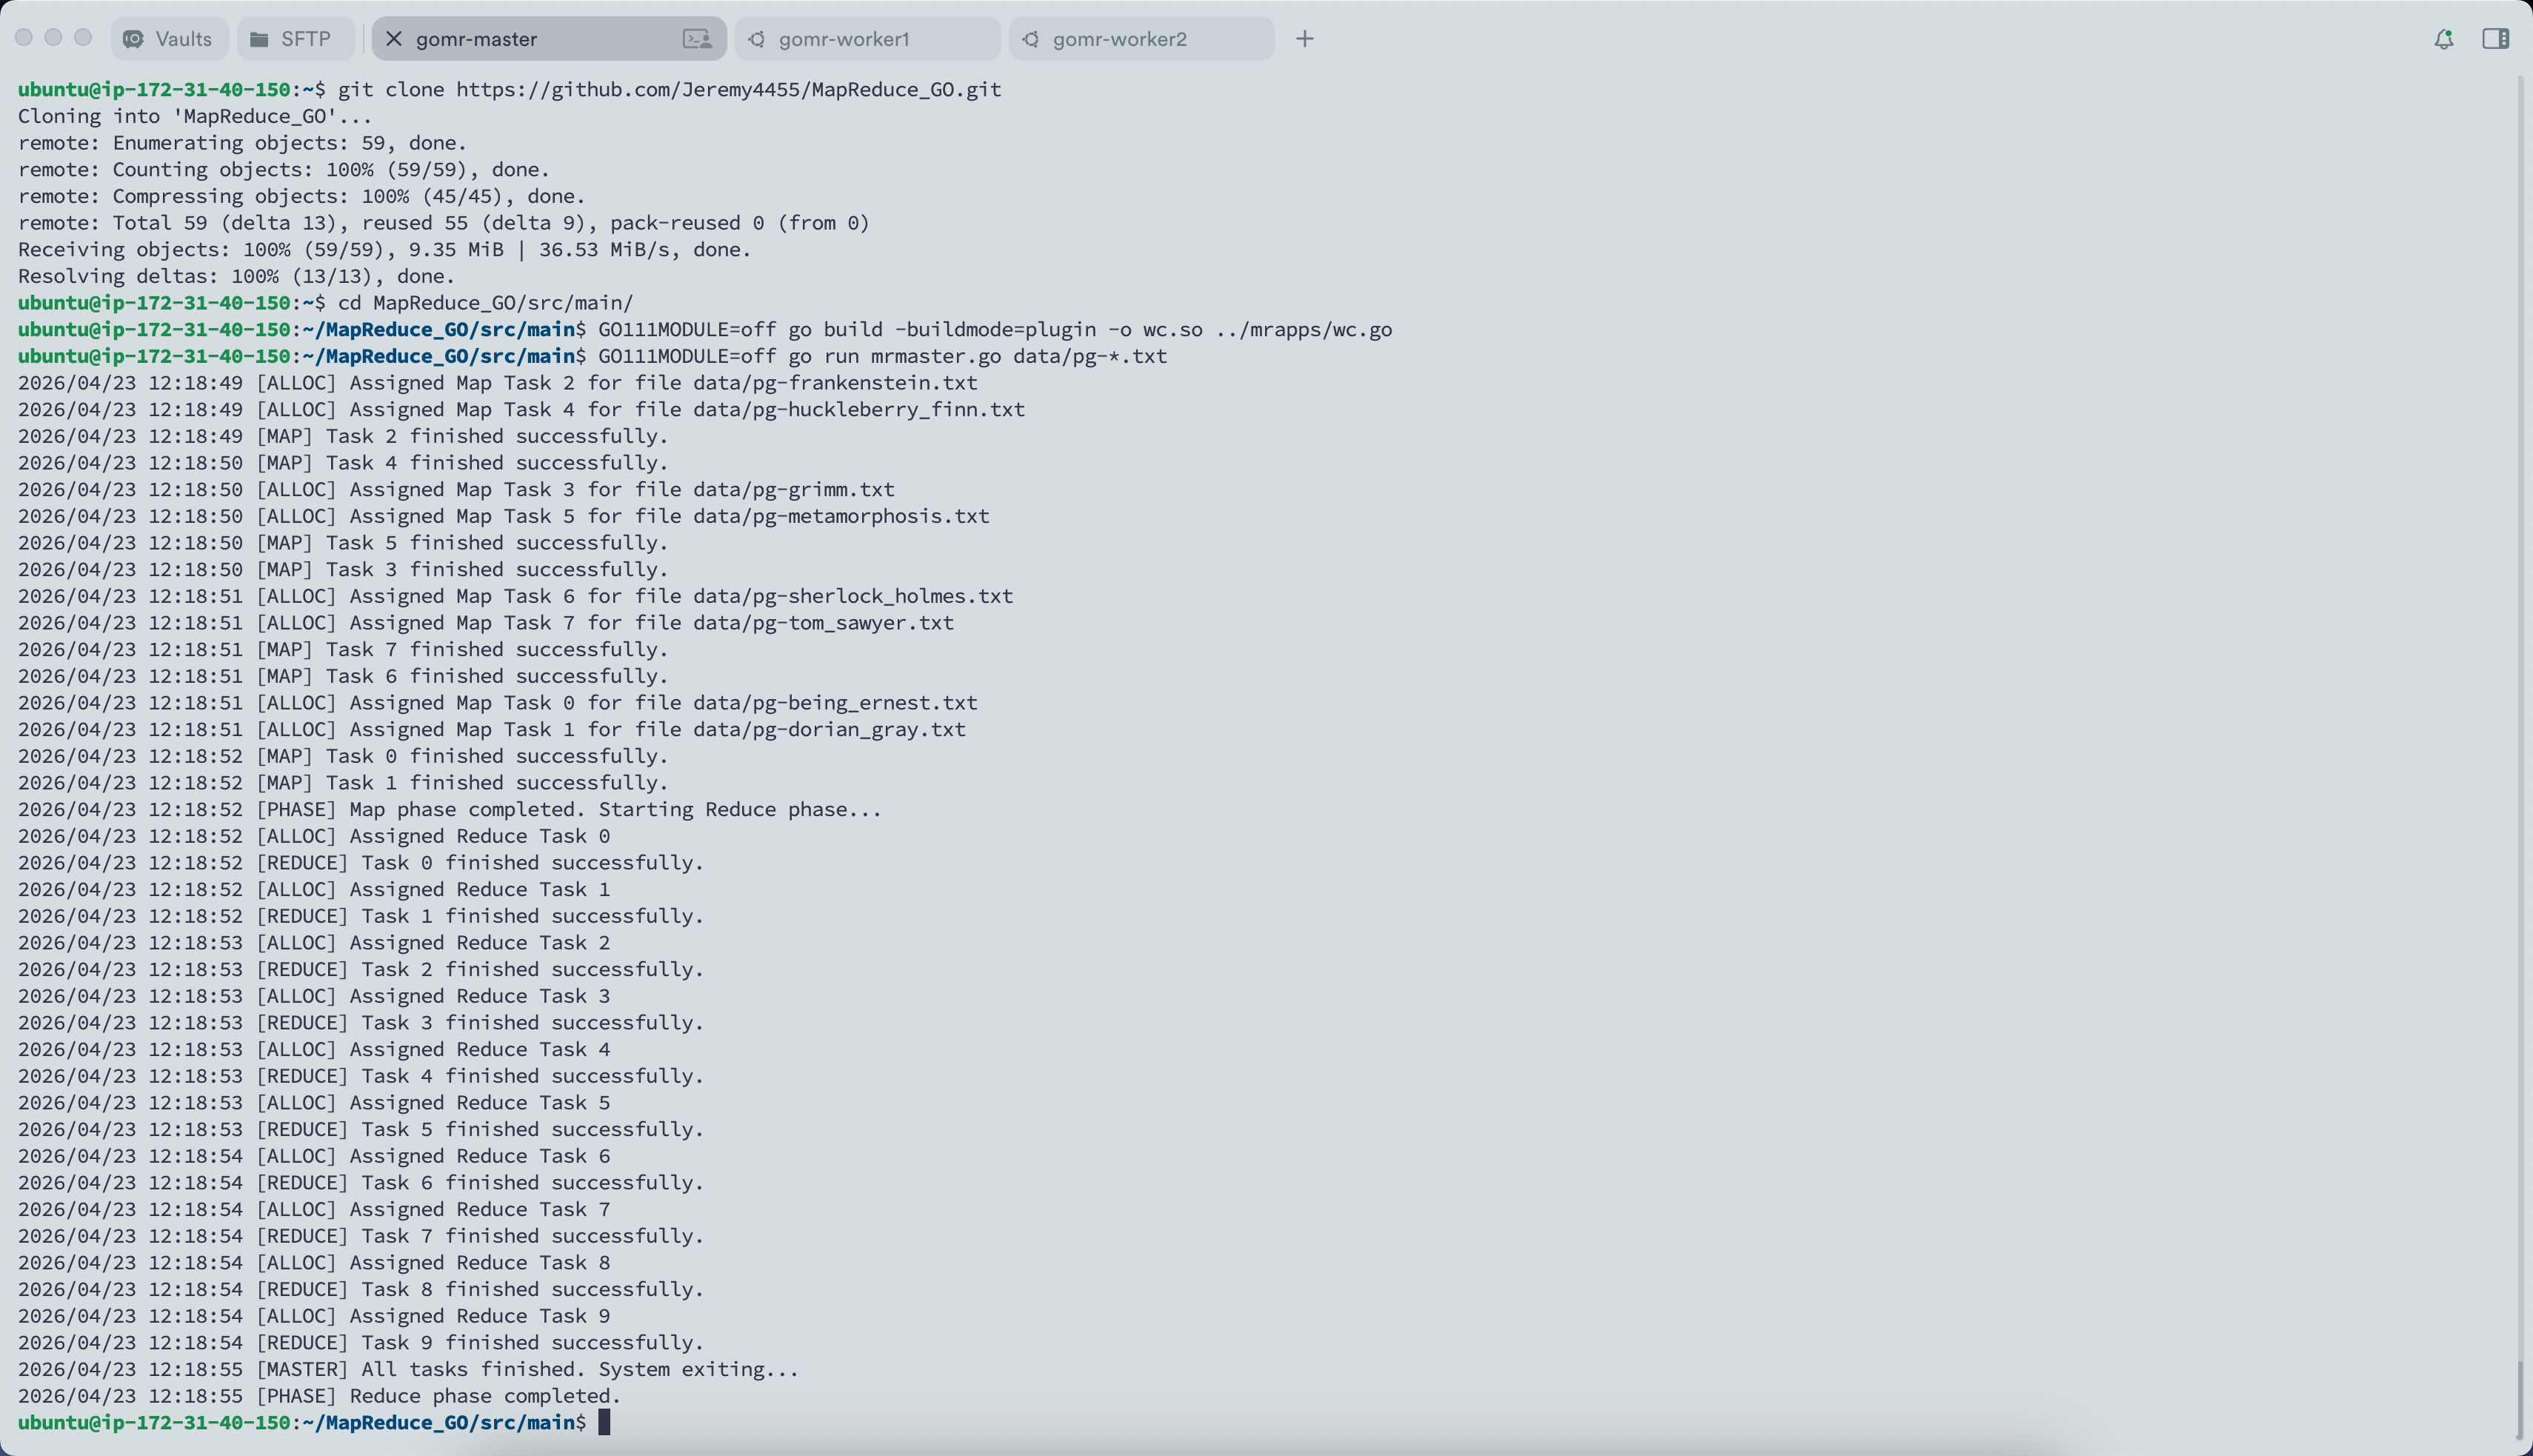
\includegraphics[width=0.85\textwidth]{assets/images/master.png}
\caption{Master-side evidence of scheduling correctness: dynamic task allocation, map-to-reduce phase transition, timeout detection, and task reallocation until global completion.}
\label{fig:master-runtime}
\end{figure}
}{}

\IfFileExists{assets/images/worker1.png}{
\begin{figure}[H]
\centering
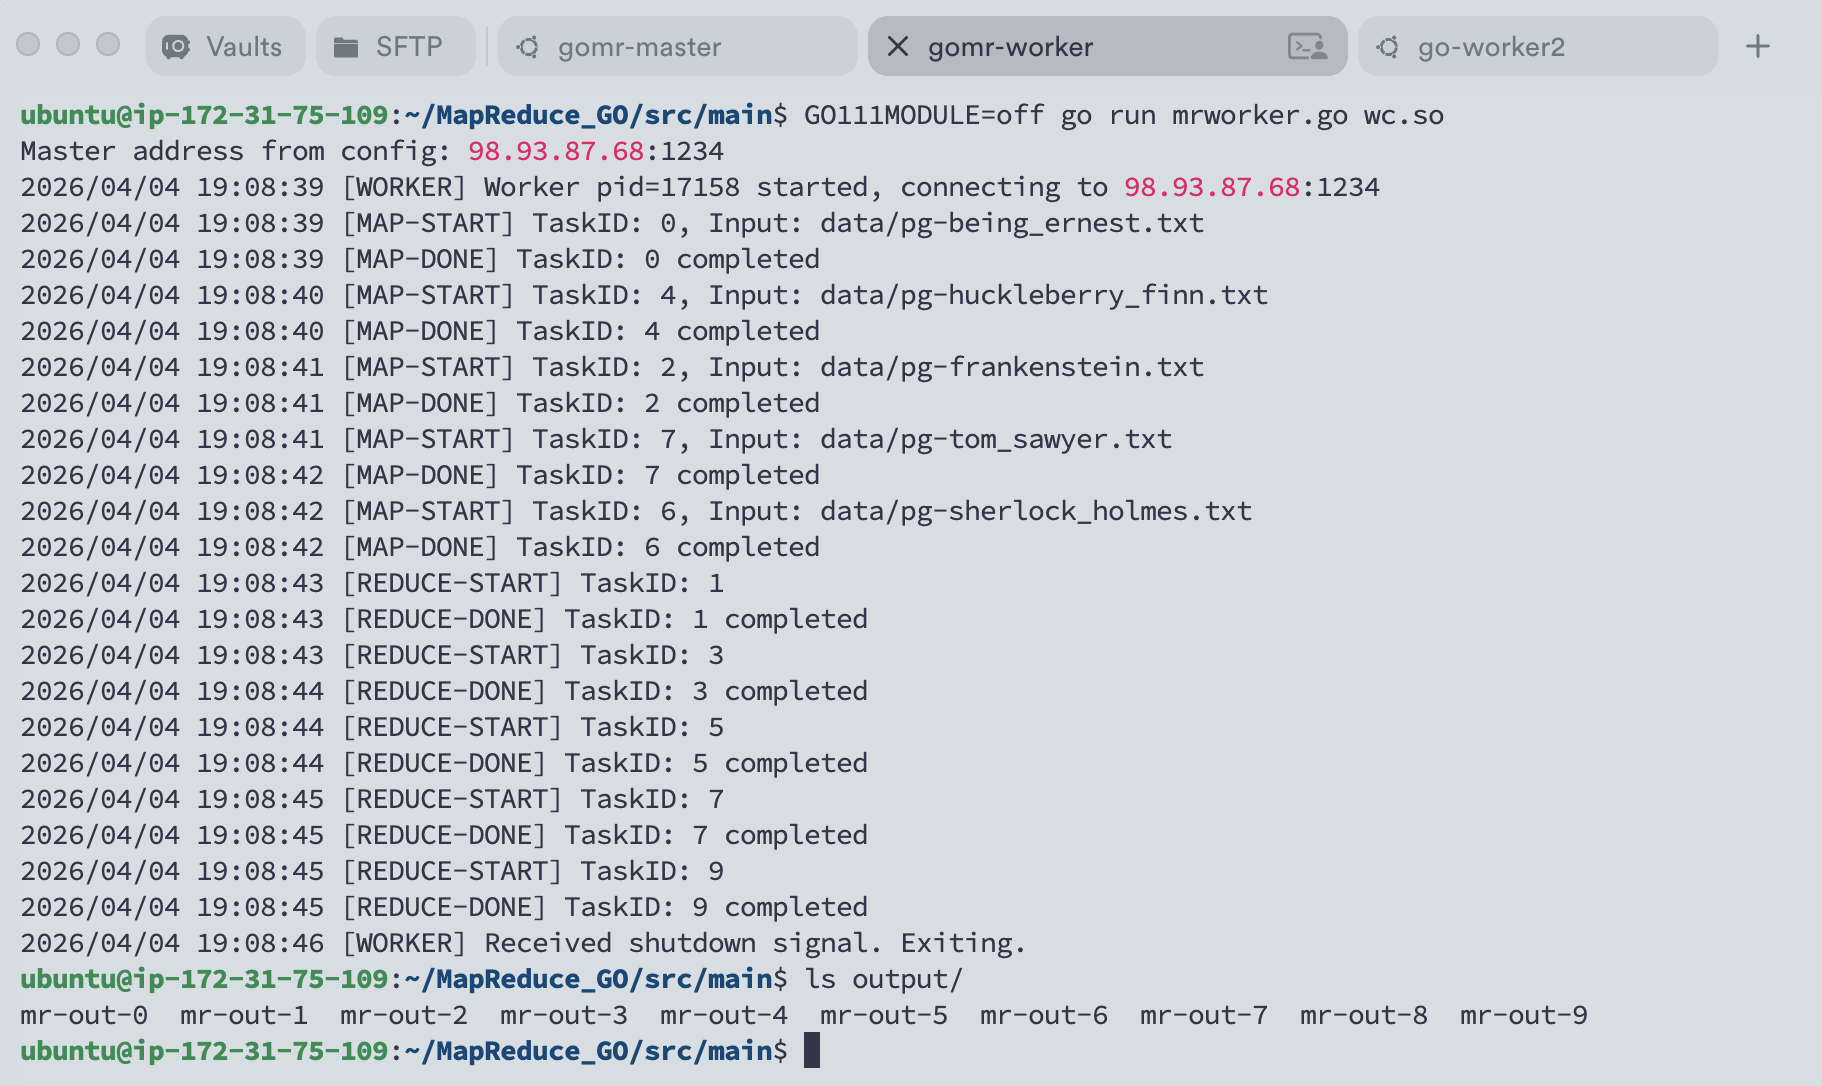
\includegraphics[width=0.85\textwidth]{assets/images/worker1.png}
\caption{Worker 1 execution evidence: successful map and reduce task processing, local intermediate output generation, and RPC-based success/failure status reporting to the master.}
\label{fig:worker1-runtime}
\end{figure}
}{}

\IfFileExists{assets/images/worker2.png}{
\begin{figure}[H]
\centering
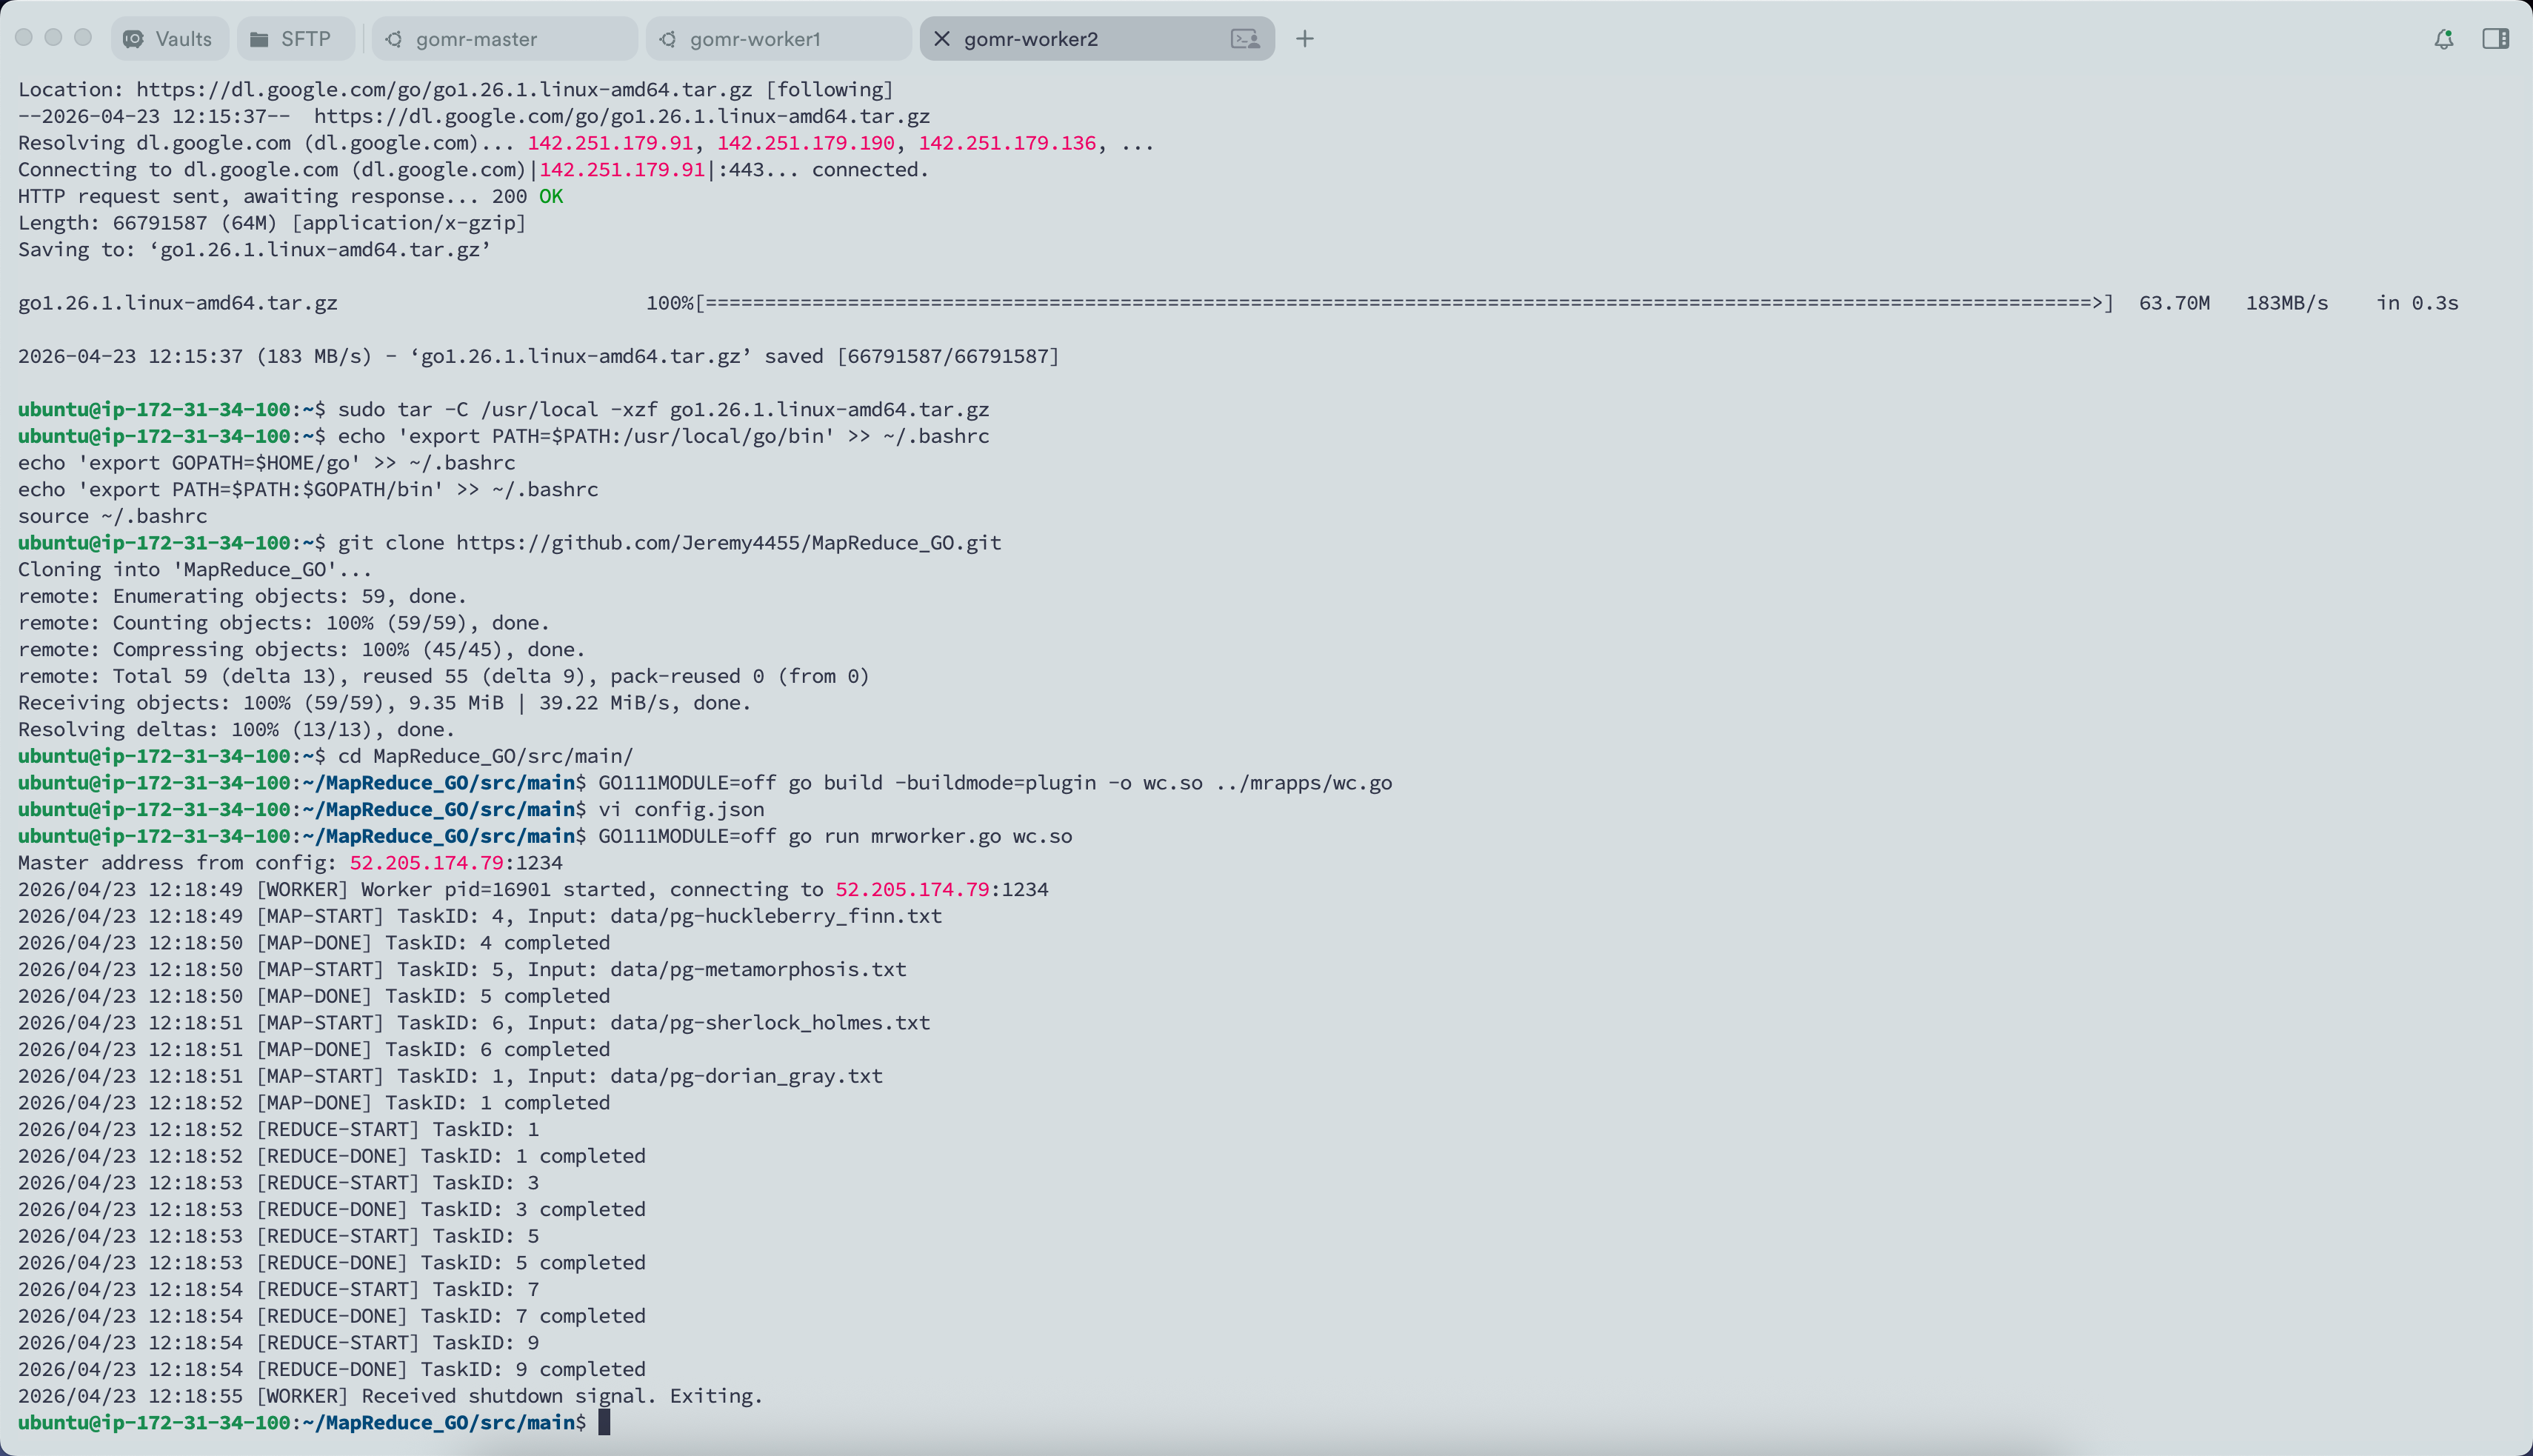
\includegraphics[width=0.85\textwidth]{assets/images/worker2.png}
\caption{Worker 2 parallelism and fault-tolerance evidence: concurrent participation in task pool, reassigned-task execution after timeout/failure, and cooperative completion with Worker 1.}
\label{fig:worker2-runtime}
\end{figure}
}{}

\subsection{Limitations}
Current evaluation is functional and qualitative. A stronger comparison against Hadoop (runtime, CPU/memory, speedup curves) remains future work and requires a controlled benchmark harness across identical cluster configurations.

\section{Conclusion}
We implemented a working MapReduce runtime in Go with dynamic task assignment, phase transition control, and basic failure recovery. The system successfully executes the full map-reduce pipeline using plugin-defined logic and generates reproducible WordCount results on multi-file text datasets. The project demonstrates key distributed systems concepts in a compact codebase and provides a practical foundation for further optimization. Future work includes quantitative benchmarking, stronger fault tolerance, and richer scheduling policies.

\begin{thebibliography}{9}
\bibitem{google-mapreduce}
J. Dean and S. Ghemawat, ``MapReduce: Simplified Data Processing on Large Clusters,''
\emph{Communications of the ACM}, vol. 51, no. 1, pp. 107--113, 2008.

\bibitem{go-official}
The Go Authors, ``The Go Programming Language,'' \url{https://go.dev/}, accessed Apr. 2026.

\bibitem{mit6824}
MIT 6.824, ``Lab 1: MapReduce,'' \url{https://pdos.csail.mit.edu/6.824/labs/lab-mr.html}, accessed Apr. 2026.

\bibitem{gutenberg}
Project Gutenberg, ``Free eBooks,'' \url{https://www.gutenberg.org/}, accessed Apr. 2026.
\end{thebibliography}

\appendix
\section*{Artifact Appendix}
\addcontentsline{toc}{section}{Artifact Appendix}

\subsection*{A. Repository and Artifact Link}
\begin{itemize}[leftmargin=1.5em]
  \item GitHub repository: \url{https://github.com/Jeremy4455/MapReduce_GO}
  \item Main implementation path: \texttt{src/mr}
  \item WordCount plugin path: \texttt{src/mrapps/wc.go}
\end{itemize}

\subsection*{B. Dependencies}
\begin{itemize}[leftmargin=1.5em]
  \item OS: Linux (recommended Ubuntu)
  \item Go toolchain: version compatible with plugin mode
  \item GCC: required by Go plugin build mode
  \item Network: TCP access to master port \texttt{1234}
\end{itemize}

\subsection*{C. Build and Run}
\begin{enumerate}[leftmargin=1.5em]
  \item Enter \texttt{src/main}.
  \item (Optional cleanup) remove stale outputs:
\begin{center}
\texttt{rm -f mr-out-* \&\& rm -rf output}
\end{center}
  \item Build plugin:
\begin{center}
\texttt{GO111MODULE=off go build -buildmode=plugin -o wc.so ../mrapps/wc.go}
\end{center}
  \item Start master:
\begin{center}
\texttt{GO111MODULE=off go run mrmaster.go data/pg-*.txt}
\end{center}
  \item Start one or more workers:
\begin{center}
\texttt{GO111MODULE=off go run mrworker.go wc.so}
\end{center}
\end{enumerate}

\subsection*{D. Expected Outputs}
\begin{itemize}[leftmargin=1.5em]
  \item Intermediate files: \texttt{mr-out-X-Y}
  \item Final results: \texttt{output/mr-out-*} (10 files for \texttt{NReduce=10})
  \item Master completion log: \texttt{All tasks finished}
\end{itemize}

\subsection*{E. Validation}
Basic validation command:
\begin{center}
\texttt{cat output/mr-out-* | sort -k2nr | head -n 10}
\end{center}
Expected behavior: frequent words (e.g., stop words) appear with high counts; repeated runs with the same input produce consistent totals.

Additional consistency checks:
\begin{center}
\texttt{ls output/mr-out-* | wc -l}
\end{center}
Expected value: \texttt{10}.

\begin{center}
\texttt{cat output/mr-out-* | awk '\{s+=\$2\} END \{print s\}'}
\end{center}
Expected behavior: total token count is deterministic across repeated runs on the same dataset.

\subsection*{F. Portable Workflow Notes}
The artifact can be reproduced directly with the command sequence above on Linux with Go+GCC installed. A container/VM image is not included in the current repository snapshot. For stronger portability, we recommend adding one of the following:
\begin{itemize}[leftmargin=1.5em]
  \item a Dockerfile that builds \texttt{wc.so} and starts master/worker processes, or
  \item a shell script (e.g., \texttt{run\_all.sh}) that automates cleanup, build, launch, and validation.
\end{itemize}

\subsection*{G. Notes for Reviewers}
\begin{itemize}[leftmargin=1.5em]
  \item If plugin loading fails, confirm Go/GCC compatibility and rebuild \texttt{wc.so}.
  \item If workers cannot connect, check \texttt{config.json} and firewall/security group settings.
  \item Re-run experiments after cleaning stale \texttt{mr-out-*} files.
  \item The current repository snapshot does not include screenshot files referenced by \texttt{README.md}; verification should rely on logs and generated outputs.
\end{itemize}

\end{document}
